\documentclass[12pt, 
hyperref={colorlinks=true, linkcolor=blue, urlcolor=cyan},dvipsnames]{beamer}
\usetheme{default} 

\setbeamertemplate{navigation symbols}{} %gets rid of navigation symbols
\setbeamertemplate{footline}{} %gets rid of bottom navigation bars
\setbeamertemplate{footline}[page number]{} %use this for page numbers

\setbeamertemplate{itemize items}[circle] %round bullet points
\setlength\parskip{10pt} % white space between paragraphs

\usepackage{wrapfig}
\usepackage{subfig}
\usepackage{setspace}
\usepackage{enumerate}
\usepackage{graphicx}
\usepackage{amsmath}
\usepackage{amsfonts}
\usepackage{amssymb}
\usepackage{amsthm}
\usepackage[UKenglish]{isodate}
\usepackage{verbatim}
\usepackage{xcolor}
\cleanlookdateon

% new amber color
\definecolor{amber}{rgb}{1.0, 0.75, 0.0}

\DeclareMathOperator{\argmin}{argmin}

% the preamble
\title{BIOST 311: \\ Regression Methods for the Health Sciences}
\author{Kelsey Grinde and Brian Williamson}
\institute{UW Biostatistics}
\date{Spring 2018}

\begin{document}
% title slide
\begin{frame}
\titlepage\thispagestyle{empty}
\end{frame}

% make it 1.something
\setbeamertemplate{footline}{%
  \raisebox{5pt}{\makebox[\paperwidth]{\makebox[120pt]{\scriptsize Last updated \today}\hfill\makebox[20pt]{\scriptsize 3.\insertframenumber~~}}}}  \newcounter{chap3}{\value{1}}
\setcounter{framenumber}{\value{chap3}}

\begin{frame}
\frametitle{CHAPTER 3: SURVIVAL ANALYSIS}
By the end of Chapter 3, you should be able to: \vspace{-0.3cm}

\begin{itemize}
\item Determine if a variable has been \textcolor{BurntOrange}{right-censored}
\item Discuss the \textcolor{red}{drawbacks} of treating a right-censored variable as binary or continuous
\item \textbf{Interpret Kaplan-Meier curves}, and create them in \texttt{R}
\item \textbf{Implement and interpret} a log-rank test for equating survival curves
\item \textbf{Formulate a regression model} given a scientific or statistical question about a right-censored outcome
\item \textbf{Interpret the coefficients} for a (simple or multiple) proportional hazards regression model
\item \textbf{Interpret confidence intervals and p-values} for proportional hazards regression coefficients
\item Use \texttt{R} to fit a proportional hazards regression model and create figures/tables to support your regression analysis
\end{itemize}

\end{frame}

\section{Censored outcomes}
\begin{frame}
\frametitle{SECTION 1: CENSORED OUTCOMES}
Up to this point, we have focused on questions involving \textcolor{blue}{quantitative} or \textcolor{BurntOrange}{binary} outcomes: 
\begin{itemize}
\item Is lung function (\textcolor{blue}{FEV}) associated with smoking, after adjusting for age, height, and sex?
\item Is cognitive function (\textcolor{blue}{DSST score}) associated with alcohol use, adjusting for age, sex, and education?
\item Is \textcolor{BurntOrange}{diabetes} associated with BMI, after adjusting for sex?
\end{itemize}
\end{frame}

\begin{frame}
\frametitle{SECTION 1: CENSORED OUTCOMES}
However, we are often interested in scientific questions that involve \textcolor{blue}{time-to-event} outcomes:
\begin{itemize}
\item Is \textcolor{blue}{time to first seizure post operation to remove a brain tumor} associated with pre-operation case review by an epileptologist, in children with both epilepsy and brain tumor?
\item Is \textcolor{blue}{time to promotion for university faculty members} associated with sex?
\item Is \textcolor{blue}{time to death from any cause} associated with serum levels of C reactive protein?
\end{itemize}
\end{frame}

\begin{frame}
\frametitle{Characteristics of survival data}
We wish to study whether \textcolor{blue}{meditation} prolongs the \textbf{time until a severe panic attack} in patients suffering from a panic disorder.

To address this question, we: \vspace{-0.3cm}
\begin{itemize}
\item recruit 200 patients and randomize them to meditation or placebo;
\item follow each patient until their first severe panic attach post recruitment;
\item and compare the mean time until a severe panic attack in each group with a t-test
\end{itemize}

{\fontsize{10pt}{7.2}\selectfont
Sample of the observed times until first severe panic attack (in weeks):
\hspace*{-1cm}\begin{tabular}{|c|c|c|c|c|c|c|c|c|c|}
\hline
\textcolor{blue}{meditation group} & 17.78 & 13.8 & 10.69 & 4.61 & 7.8 & 26.32 & 6.48 & 12.51  \\
\hline
control group & 12.45 & 18.42 & 15.95 & 8.18 & 21.74 & 6.47 & 11.01 & 22.44 \\
\hline
\end{tabular}
}
\end{frame}

\begin{frame}
\frametitle{Characteristics of survival data}
\centering
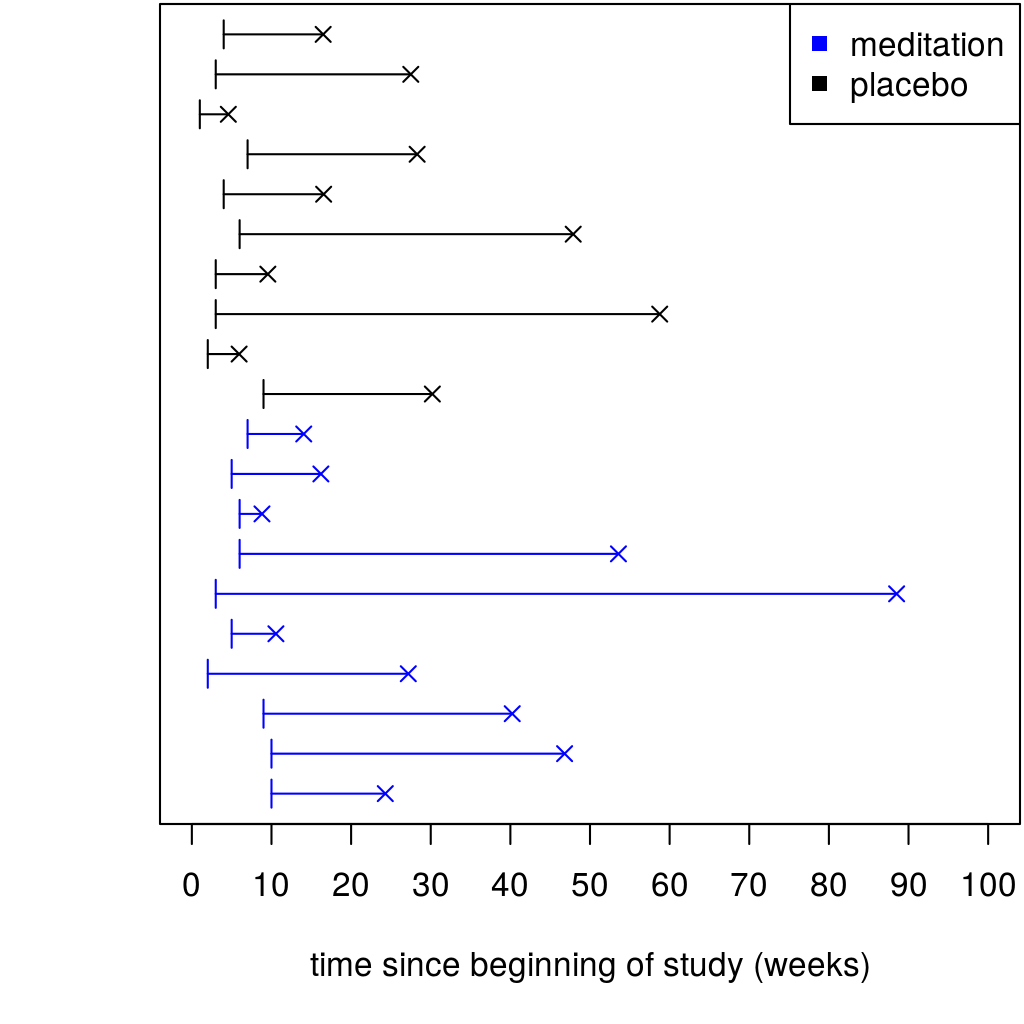
\includegraphics[width=0.8\textwidth]{figs/meditation_observed_study_time.png}
\end{frame}

\begin{frame}
\frametitle{Characteristics of survival data}
\centering
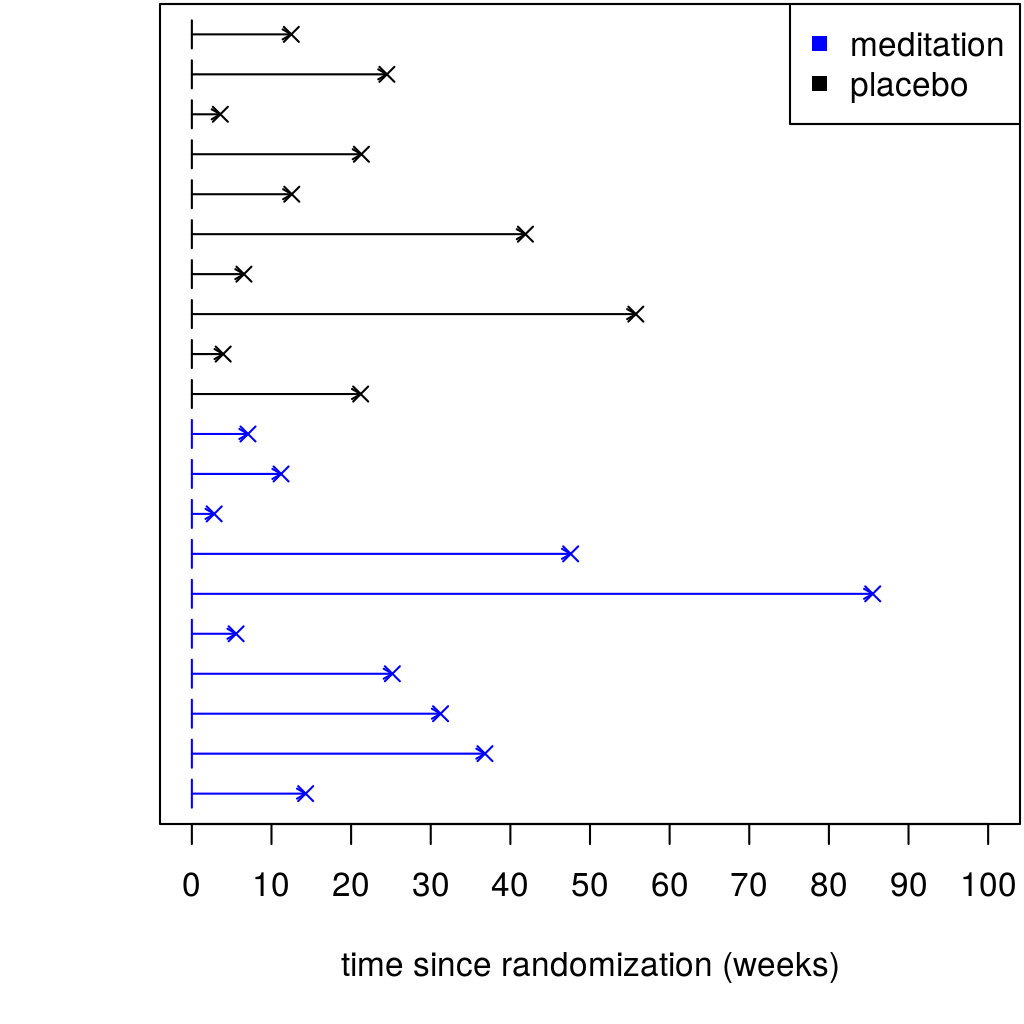
\includegraphics[width=0.8\textwidth]{figs/meditation_observed_rand_time.png}
\end{frame}

\begin{frame}
\frametitle{Characteristics of survival data}
In this hypothetical study, we were able to record the actual occurrence time \textcolor{blue}{for each participant}.

Is this typical of human studies? \pause \textcolor{red}{No!}

Why? \pause Some common reasons are:
\begin{itemize}
\item the study ended (e.g., after 30 weeks) and some participants had not yet had a severe panic attack (\textbf{administrative censoring})
\item the participant left the study before having had a severe panic attack (\textbf{loss to follow-up})
\end{itemize}

These all lead to \textbf{right-censored} data, where rather than knowing the value exactly, we know that the value exceeds some cutoff.
\end{frame}

\begin{frame}
\frametitle{Characteristics of survival data}
\centering
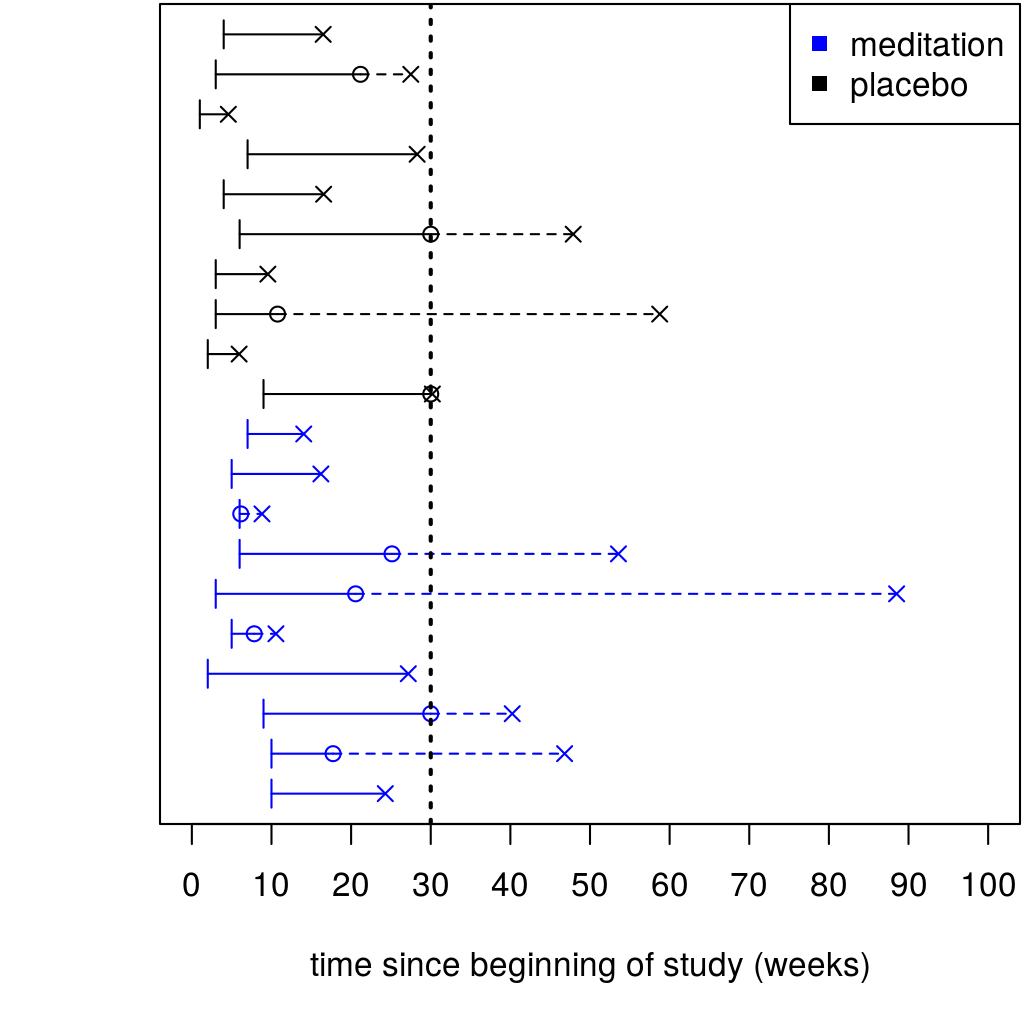
\includegraphics[width=0.8\textwidth]{figs/meditation_censored_study_time.png}
\end{frame}

\begin{frame}
\frametitle{Characteristics of survival data}
\centering
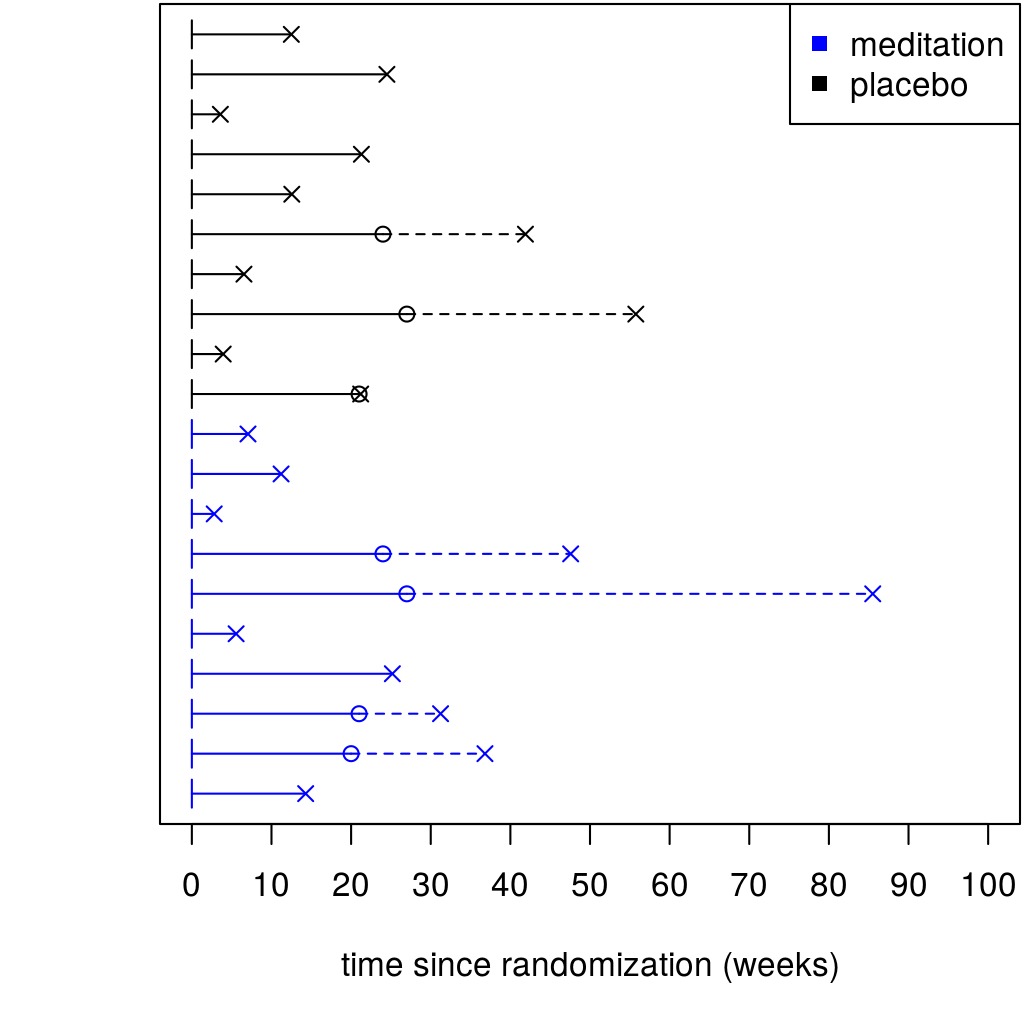
\includegraphics[width=0.8\textwidth]{figs/meditation_censored_rand_time.png}
\end{frame}

\begin{frame}
\frametitle{Characteristics of survival data}
{\fontsize{10pt}{7.2}\selectfont
The data can be represented as:
\hspace*{-1cm}\begin{tabular}{|c|c|c|c|c|c|c|c|c|c|}
\hline
\textcolor{blue}{meditation group} & 14.29  & \textcolor{red}{7.74+} & \textcolor{red}{21.00+} & 25.18  &  \textcolor{red}{2.83+} & \textcolor{red}{17.57+} & \textcolor{red}{19.13+} &  \textcolor{red}{0.14+}  \\
\hline
control group & \textcolor{red}{21.00+} &  \textcolor{red}{3.94+} &  \textcolor{red}{7.77+} &  6.54  & \textcolor{red}{24.00+} & 12.55  & 21.29 &  3.58 \\
\hline
\end{tabular}
}

\vspace{-0.6cm}
{\small
Should we treat these incompletely observed times as missing data? Should we throw them out? \pause \textcolor{red}{Either of these is a bad idea!} \vspace{-0.3cm}

\begin{itemize}
\item These observations contain valuable information:
{\scriptsize
\begin{itemize}
\item \textcolor{red}{20+}: the participant did not experience a severe panic attack before 20 weeks
\item their actual time until the first severe panic attack must be in the interval $(20, +\infty)$
\end{itemize}
}
\item These participants are not representative of the whole study population: valid estimation and inference when excluding missing data (which we have done so far) assumes that the people excluded are ``similar to'' the people still in the data (\textbf{missing completely at random})
\end{itemize}
}
\end{frame}

\begin{frame}
\frametitle{Characteristics of survival data}
Close or put away your notes and laptops. Then answer the following questions, at first alone, and then in pairs:
\begin{enumerate}
\item Are those with smaller or larger times more likely to be censored?
\item Systematically excluding censored times could lead to \textcolor{red}{biased estimates}. Would this lead to an overestimation or an underestimation of the mean time until severe panic attack?
\end{enumerate}

\end{frame}

\begin{frame}
\frametitle{Characteristics of survival data}
\begin{enumerate}
\item Are those with smaller or larger times more likely to be censored?
\item[] \textcolor{blue}{Those with \textbf{larger times} are more likely to be censored; we only get to observe these people for a comparatively small amount of time, so we may miss their event}
\item Systematically excluding censored times could lead to \textcolor{red}{biased estimates}. Would this lead to an overestimation or an underestimation of the mean time until severe panic attack?
\item[] \textcolor{blue}{\textbf{Underestimation}: if we exclude censored times, then we are effectively excluding these people with potentially longer times, and losing all of this information!}
\end{enumerate}

\end{frame}

\begin{frame}
\frametitle{Characteristics of survival data}
Sampling distribution of times in participants who become censored or uncensored, and the overall target population:\vspace{-0.4cm}
\begin{center}
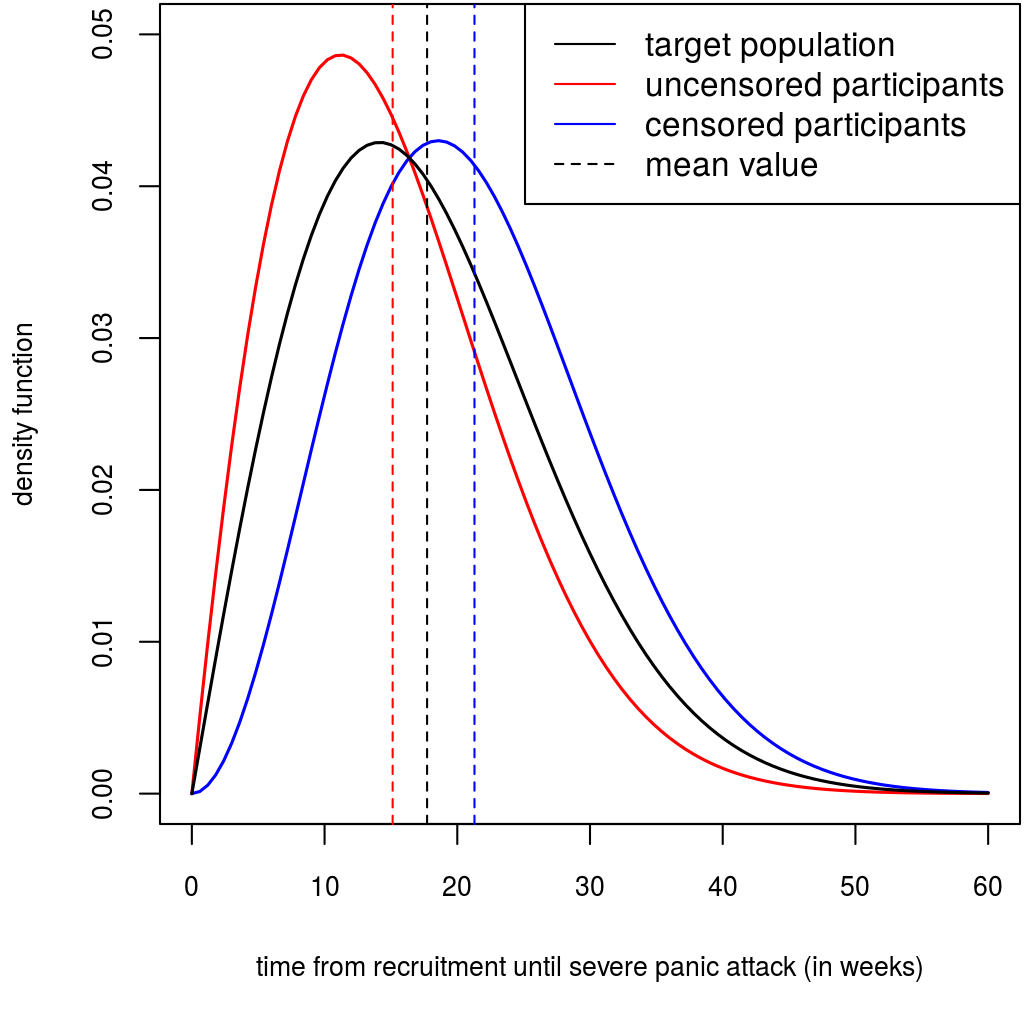
\includegraphics[height=0.8\textheight]{figs/meditation_density_versus_obs_time.png}
\end{center}
\end{frame}

\begin{frame}
\frametitle{Characteristics of survival data}
\textbf{Survival analysis} is the branch of statistics concerned with the analysis of \textbf{time-to-event data}.

Often, the goals of a survival analysis are to:
\begin{itemize}
\item describe the distribution of a time-to-event variable
\item compare the time-to-event distribution in different subpopulations
\item investigate the relationship between explanatory variables and the time-to-event distribution
\end{itemize}
\end{frame}

\begin{frame}
\frametitle{Characteristics of survival data}
Why is time-to-event data special? Why can we not use standard methods? \vspace{-0.5cm}
\begin{itemize}
\item A time-to-event variable is positive and generally skewed
\item To appropriately define a time-to-event, we must specify:
{\scriptsize
\begin{itemize}
\item initiating event --- e.g., birth, recruitment into study, onset of disease
\item terminating event --- e.g., death, onset of disease
\item time scale --- e.g., calendar time, number of transfusions
\end{itemize}
}
\item Time-to-event data are generally observed subject to some incompleteness, of which \textbf{censoring} is a major type
\item Throwing away incomplete data generally results in
{\scriptsize
\begin{enumerate}
\item a loss of information (and increase in estimation uncertainty)
\item biased estimation procedures (most important!)
\end{enumerate}
}
\end{itemize}

\end{frame}

\begin{frame}
\frametitle{Characteristics of survival data}
A time-to-event variable is said to be \textbf{censored} if rather than being known exactly, it is known to lie in some set of values.

In this course, we will focus on \textbf{right censoring}, where we only know that the event occurred after the censoring point.

Right-censored data are the most common type of censored data found in applications!
\end{frame}

% risk set, plus movie
\begin{frame}
\frametitle{Characteristics of survival data}
Key concept: the \textbf{risk set}.

\textbf{Risk set at time $t$}: the collection of participants \textcolor{blue}{could have experienced} their first severe panic attack at time $t$; in other words, those who were still at risk at time $t$.
\vspace{-0.3cm}
\begin{align*}
\textbf{fraction at risk at time } t = & \frac{\textbf{size of risk set at time } t}{\textbf{total sample size}}.
\end{align*}

A few observations:\vspace{-0.3cm}
\begin{itemize}
\item participants \textcolor{blue}{exit} the risk set either when they \textcolor{Aquamarine}{experience a severe panic attack} or when they \textcolor{red}{become right-censored}
\item with right-censored data, all participants are in the risk set at time 0 and the risk set necessarily shrinks over time
\item the \textcolor{blue}{size of the risk set} and the \textcolor{blue}{characteristics of its members} will be critical in survival analysis
\end{itemize}
\end{frame}

\begin{frame}
\frametitle{Characteristics of survival data}

\end{frame}

% uninformative censoring, with examples (from Anna)

% key quantities: density function, survival function, hazard function


\begin{comment}
\section{Nonparametric estimation and inference}
\begin{frame}
\frametitle{SECTION 2: NONPARAMETRIC ESTIMATION}
\end{frame}

\section{Semiparametric estimation and inference}
\begin{frame}
\frametitle{SECTION 3: SEMIPARAMETRIC ESTIMATION}
\end{frame}
\section{Summary}
\begin{frame}
\frametitle{SECTION 4: SUMMARY}
\end{frame}
\end{comment}
\end{document}